\chapter{ROM Results: MVAR vs LSTM}
\label{ch:rom_results}

This chapter presents the reduced-order modelling results for MVAR and LSTM~\cite{hochreiter1997lstm}
applied to the equation-free density ROM\@.  The \emph{primary benchmark}
comprises five constant-speed (CS) regimes plus a pure alignment
baseline (\texttt{NDYN04\_gas}, \texttt{NDYN05\_blackhole},
\texttt{NDYN06\_supernova}, \texttt{NDYN07\_crystal}, and
\texttt{NDYN08\_pure\_vicsek}), which
span the key behavioural axes (attraction, repulsion, equilibrium,
alignment only)
under well-controlled shift dynamics.  In addition, four
\emph{variable-speed} (VS) diagnostic variants (\texttt{NDYN04\_gas\_VS},
\texttt{NDYN05\_blackhole\_VS}, \texttt{NDYN06\_supernova\_VS}, and
\texttt{NDYN07\_crystal\_VS}) are
included to test whether the performance ceiling observed on the primary
benchmark is a \emph{structural} limitation of single-reference sPOD~\cite{reiss2018shifted_pod} or
merely a model-class limitation that a more expressive forecaster could
overcome.  Aggregate statistics reported in this chapter (median $R^2$,
efficiency comparisons) are computed over the CS\,+\,PV primary benchmark
unless stated otherwise; VS results are presented as a separate diagnostic.
The complete systematic catalogue with dynamics parameters and
per-regime $R^2$ is provided in Appendix~\ref{app:full_regime_catalogue},
and per-experiment supplementary figures are collected in
Appendix~\ref{app:supplementary_figures}.

% -----------------------------------------------------------------------
\section{Shift predictability as the benchmark ceiling}
\label{sec:ch7_shift_dynamics}
% -----------------------------------------------------------------------

Accordingly, the forecast task studied here is not full transport
prediction in lab coordinates, but density-shape prediction after removal
of bulk translation.

The MVAR has relatively low statistical complexity in the
aligned latent space, whereas the LSTM must estimate a substantially more
flexible temporal map from the same finite set of windows---an asymmetry
worth bearing in mind when interpreting nonlinear modelling gains.
Figure~\ref{fig:ch7_svd_decay} shows the singular-value spectra of the
aligned snapshot matrices across all nine benchmark regimes.

\begin{figure}[htbp]
\centering
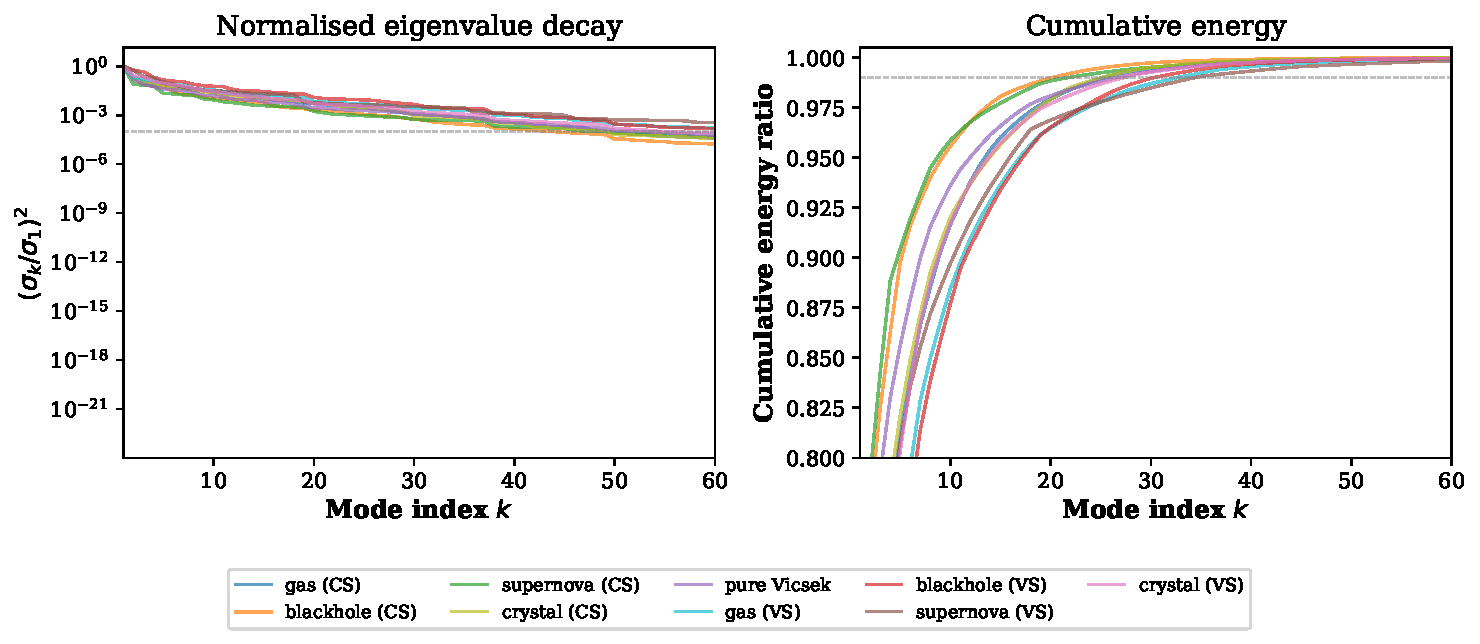
\includegraphics[width=0.92\textwidth]{../Thesis_Figures/thesis_svd_decay_ch7.pdf}
\caption{Singular-value spectra of the aligned snapshot matrices across
all nine benchmark regimes.
Left: normalised eigenvalue decay $(\sigma_k/\sigma_1)^2$ on a
log scale.  Right: cumulative energy ratio.  Each coloured curve represents
one regime.  The aligned spectra exhibit rapid decay and support a compact
POD truncation.}
\label{fig:ch7_svd_decay}
\end{figure}

Before comparing model outputs it is instructive to characterise the
difficulty of the forecasting task itself.  Both MVAR and LSTM operate
exclusively in the \emph{aligned} latent space: their state vectors are
the $r{=}19$ POD coefficients of the shift-corrected density field, and
the spatial shift $\boldsymbol{\Delta}(t)=(\Delta x(t),\,\Delta y(t))$ is
\emph{not} included as a forecast variable.  During evaluation,
ground-truth test shifts (computed via FFT cross-correlation against the
training reference frame) are used solely to un-align predictions back to
physical space for visualisation; the $R^2$ metric is computed entirely in
the aligned frame.  The temporal predictability of
$\boldsymbol{\Delta}$ nevertheless imposes a structural ceiling on
forecast fidelity: when shifts are poorly predictable the aligned density
retains residual transport structure that inflates the effective latent
dimension and degrades both models equally.
Figure~\ref{fig:ch7_phase_dynamics}
summarises two complementary shift diagnostics (trajectory geometry
and autocorrelation structure) across the benchmark regimes.

\begin{figure}[htbp]
\centering
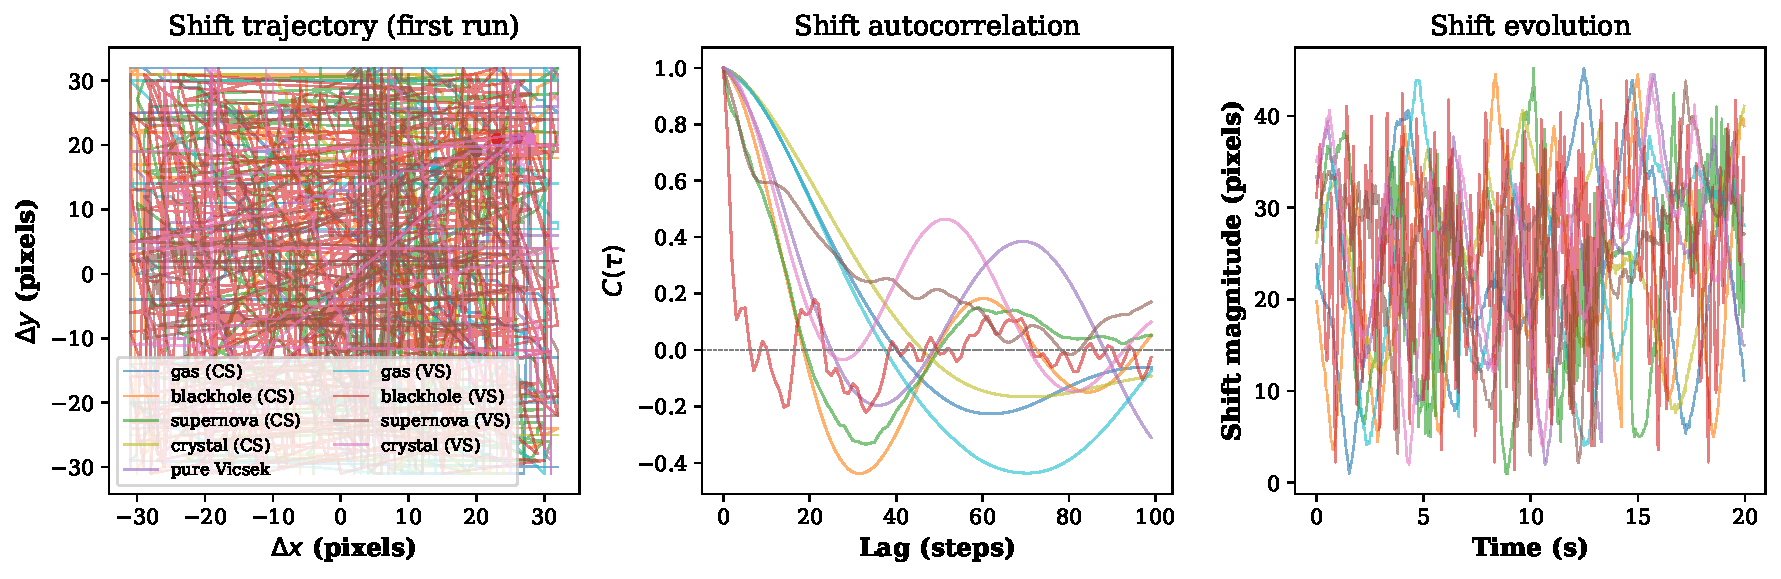
\includegraphics[width=0.92\textwidth]{../Thesis_Figures/thesis_phase_dynamics_ch7.pdf}
\caption{Shift dynamics across the benchmark regimes.
\emph{Left:} Shift trajectory $(\Delta y(t),\,\Delta x(t))$ in the
alignment frame for a representative simulation run.  Each coloured
path traces the bulk centre-of-mass displacement; symbols mark the start.
\emph{Centre:} Temporal autocorrelation $C(\tau)$ of the shift signal as a
function of lag~$\tau$, normalised so that $C(0)=1$.
\emph{Right:} Shift magnitude evolution over time, showing the raw
displacement signal $\|\boldsymbol{\Delta}(t)\|$ for each regime.
}
\label{fig:ch7_phase_dynamics}
\end{figure}

\noindent\textbf{Mean shift trajectory.}
The left panel traces $\overline{\boldsymbol{\Delta}}(t)$ in the
$(\Delta y,\Delta x)$ plane.  All regimes stay within $\pm 4$--$6$ grid
cells; gas and pure Vicsek~\cite{vicsek1995vicsek} trace smooth persistent loops, whereas
variable-speed blackhole traces a near-memoryless random walk---indicating
that bulk translation is no longer a sufficient coherent-motion summary.

\noindent\textbf{Shift autocorrelation.}
The centre panel plots the temporal autocorrelation $C(\tau)$ and partitions
regimes into three tiers: gas, supernova, and pure Vicsek retain significant
correlation at long lags; constant-speed blackhole sits intermediate;
variable-speed blackhole collapses to near-zero correlation within a few lag
steps.  The right panel shows the raw shift magnitude over time, confirming
that VS regimes exhibit faster, less structured fluctuations.
Fitting AR($p$) models ($p=1,\ldots,10$) to the shift time series
(not shown) yields consistent rankings: gas and pure Vicsek reach
$R^2\!\approx\!0.88$; supernova and constant-speed blackhole land near
$0.83$; variable-speed blackhole is a clear outlier at $\approx\!0.45$.
$R^2$ is flat across lag orders, validating the MVAR lag window
(Section~\ref{ch:latent_rom}).

\noindent\textbf{Synthesis.}
Shift predictability is a major structural determinant of ROM forecast
quality, but it is not sufficient on its own.  Variable-speed blackhole
is the clearest failure case: its shift process has the weakest temporal
structure, and LSTM falls to negative forecast~$R^2$, while MVAR remains
positive but substantially degraded.  By contrast, gas and constant-speed
blackhole combine strong shift structure with favourable aligned latent
dynamics, and both models achieve $R^2\!\approx\!0.99$.  Pure Vicsek
retains relatively predictable shifts, but its density dynamics remain
harder than gas/blackhole after alignment, so MVAR drops to moderate
rather than near-perfect accuracy.

Post-hoc eigenvalue rescaling
(Equation~\ref{eq:eigenvalue_projection}, Section~\ref{sec:ch7_stability})
clips 2--3 eigenvalues in the VS variants yet residual error remains high,
confirming that the root cause is shift autocorrelation, not linear
instability of the fitted propagator.  VS rescaling does not fix the
failure.

% -----------------------------------------------------------------------
\section{Forecasting results: qualitative and quantitative}
\label{sec:ch7_forecasting_results}
% -----------------------------------------------------------------------

This section presents the forecast evidence in three complementary views:
density snapshots illustrating spatial fidelity, aggregate $R^2$ metrics
quantifying regime-level accuracy, and order parameter trajectories testing
whether physically meaningful collective statistics survive the
compress--evolve--lift cycle.

\subsection*{Density snapshots}
\label{sec:ch7_qualitative}

We show a single representative regime (gas) where both models
succeed; additional regimes (blackhole, supernova) are collected in
Appendix~\ref{app:supplementary_figures}
(Figure~\ref{fig:appE_snapshots_blackhole}).

\begin{figure}[htbp]
\centering
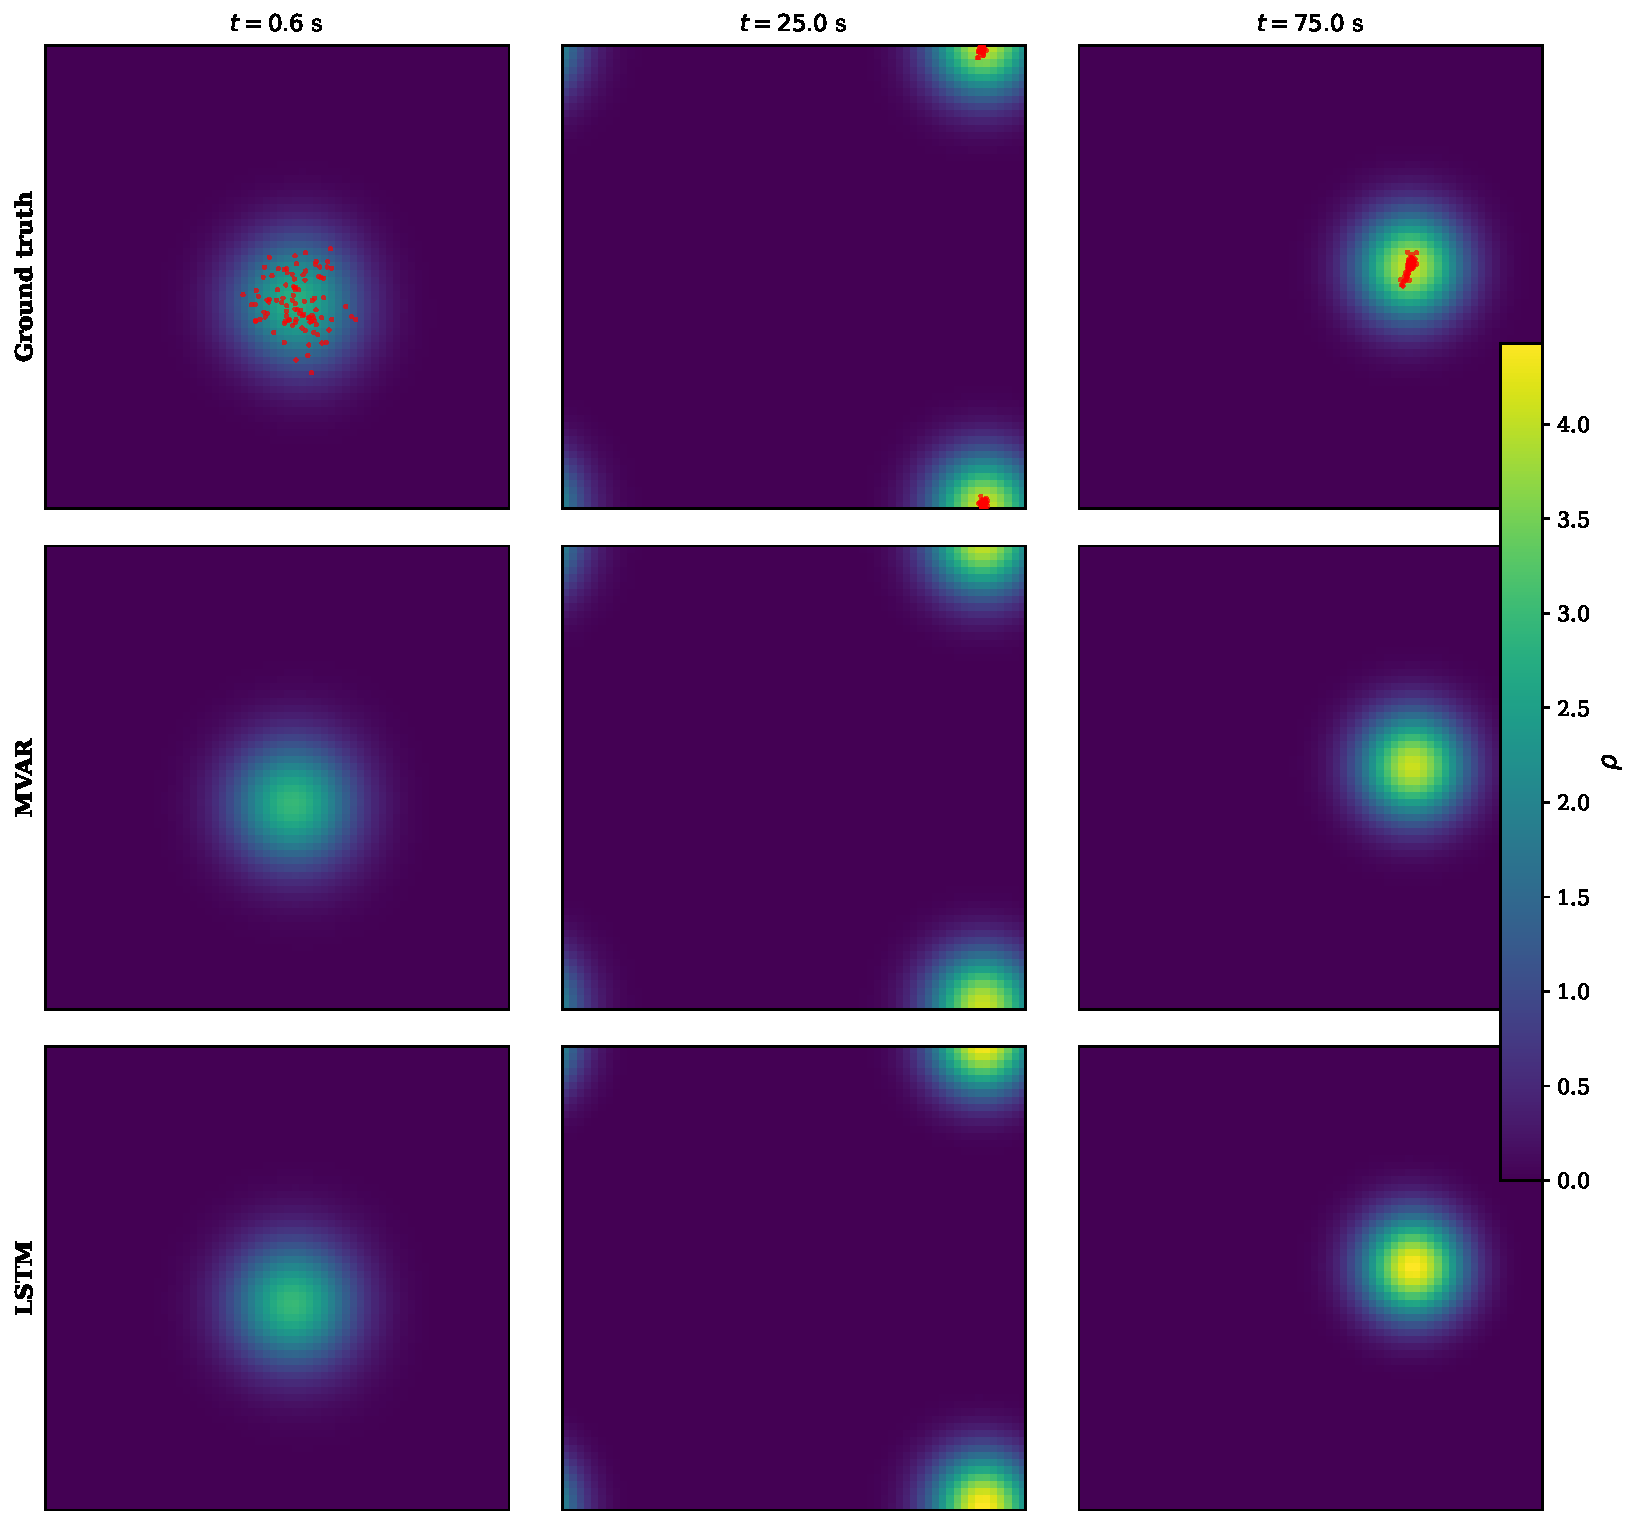
\includegraphics[width=0.92\textwidth]{../Thesis_Figures/ch7_snapshots_gas.pdf}
\caption{Density snapshots truth vs.\ prediction for
\texttt{NDYN04\_gas} (Gaussian IC, test run~0).  Columns show $t=0.6$\,s,
$t=25$\,s, and $t=75$\,s.  Rows: ground truth, MVAR, LSTM\@.  Colour scale
is shared across all panels within each time column but differs between
columns (the peak density decreases as the cluster diffuses; compare
colourbar ranges across columns).  MVAR faithfully
reproduces the diffusing cluster throughout the horizon.  LSTM maintains
gross spatial structure but develops small-scale artefacts by $t=75$\,s,
consistent with its higher variance in the $R^2(t)$ curves.}
\label{fig:ch7_snapshots_gas}
\end{figure}

Across all regimes, both forecasters reproduce the dominant low-rank
structure of the aligned density field (large-scale envelope,
centre-of-mass location, overall mass distribution) but differ in how
they handle fine-scale spatial detail and late-horizon accuracy.
MVAR's linear dynamics produce spatially smooth predictions that degrade
gracefully; LSTM's nonlinear capacity allows it to track sharper
features at the cost of occasional high-frequency artefacts once the
autoregressive rollout accumulates error.

\subsection*{Forecast $R^2$ across regimes}
\label{sec:ch7_quantitative}

\begin{figure}[htbp]
\centering
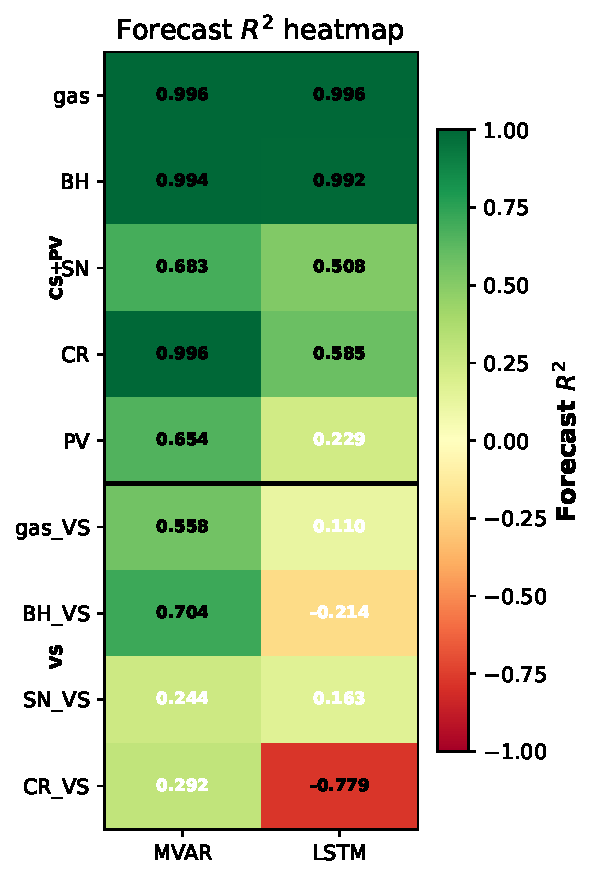
\includegraphics[width=0.82\textwidth]{../Thesis_Figures/thesis_r2_heatmap}
\caption{Forecast $R^2$ heatmap: rows are experiments (grouped by regime
family), columns are MVAR and LSTM\@.  Cell colour encodes forecast $R^2$
on a diverging red--yellow--green scale; numeric annotations give the exact
value.  A horizontal rule separates the primary benchmark (CS\,+\,PV,
top) from the VS diagnostic regimes (bottom).  WSINDy is omitted because
it produces identification-quality scores (weak-form $R^2$) rather than
time-stepped forecasts; its metrics appear in
Table~\ref{tab:wsindy_vs_efrom}.}
\label{fig:ch7_r2_heatmap}
\end{figure}

\begin{figure}[htbp]
\centering
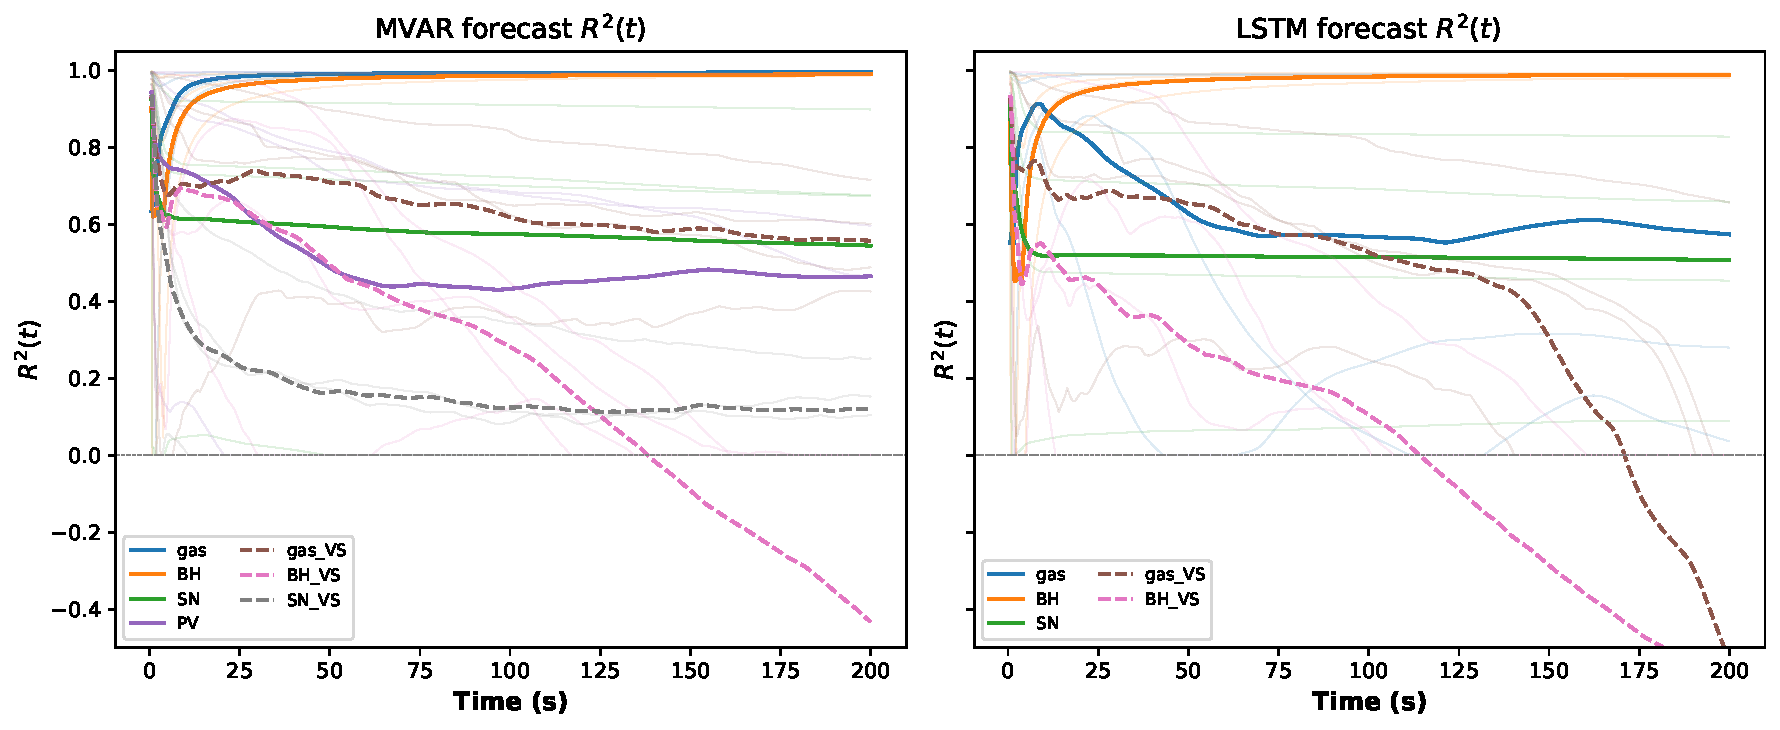
\includegraphics[width=\textwidth]{../Thesis_Figures/thesis_r2_degradation}
\caption{Forecast $R^2$ degradation over the prediction horizon
(left: MVAR, right: LSTM).  Bold curves show per-regime means; faint
traces are individual test runs.  Solid lines = CS\,+\,PV benchmarks;
dashed = VS diagnostics.  Per-experiment detail with $\pm 1\sigma$
shading is in Appendix~\ref{app:full_regime_catalogue}
(Figure~\ref{fig:appF_r2_degradation_combined}).}
\label{fig:ch7_r2_degradation}
\end{figure}

\begin{figure}[htbp]
\centering
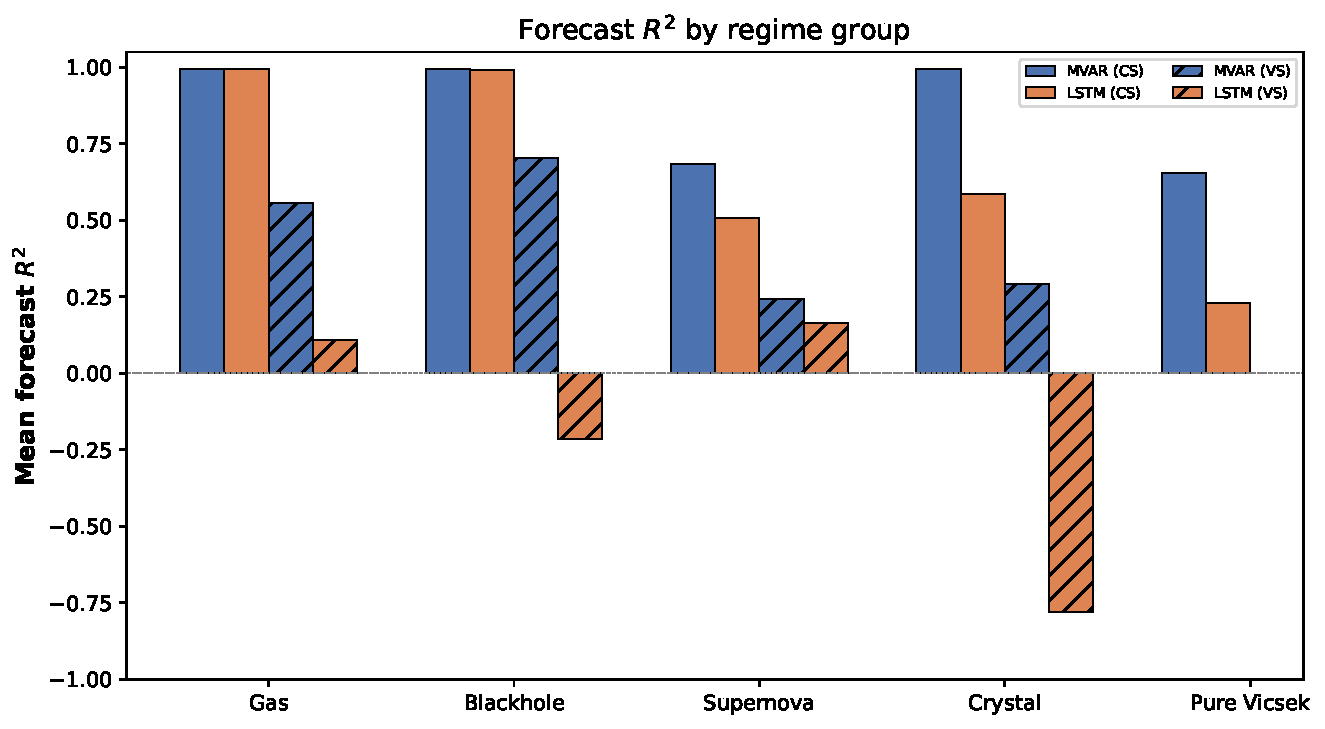
\includegraphics[width=\textwidth]{../Thesis_Figures/thesis_r2_by_group}
\caption{Mean test $R^2$ by regime group (grouped bar chart).  Each cluster
of bars corresponds to one of the five benchmark regimes
(gas, blackhole, supernova, crystal, pure Vicsek); within each
cluster, bars represent MVAR and LSTM\@.  Error bars show $\pm 1$ standard
deviation across experiments within the group.  Solid bars are the
CS\,+\,PV primary benchmark; hatched bars are the VS diagnostic
variants (pure Vicsek has no VS variant by construction).
The CS--VS gap is immediately visible and consistent across
all regime families, indicating that the bottleneck is the
shift-predictability prerequisite rather than the model class.}
\label{fig:ch7_r2_by_group}
\end{figure}

The heatmap (Figure~\ref{fig:ch7_r2_heatmap}) provides the
bird's-eye view: MVAR achieves $R^2>0.95$ on gas
and blackhole (CS), drops to roughly $0.65$--$0.68$ on supernova and pure
Vicsek, and maintains positive $R^2$ across all CS\,+\,PV regimes.  LSTM
follows a broadly similar pattern but with higher variance.
The $R^2(t)$ degradation curves
(Figure~\ref{fig:ch7_r2_degradation}) reveal that the model gap is
predominantly a late-horizon effect.

The VS diagnostic regimes show substantially reduced $R^2$ relative
to their CS counterparts.  MVAR remains positive across all VS
regimes (median $0.425$; blackhole\_VS reaches $0.704$), while LSTM
stays positive on gas\_VS ($0.11$) and supernova\_VS ($0.16$) but
falls negative on blackhole\_VS ($-0.21$) and crystal\_VS ($-0.78$).
The consistent CS--VS gap
across all interaction families
(Figure~\ref{fig:ch7_r2_by_group}) confirms that the ceiling is set by
shift predictability (Section~\ref{sec:ch7_shift_dynamics}), not
forecaster capacity.

\paragraph{Summary of quantitative findings.}
MVAR dominates the CS\,+\,PV primary benchmark (median
$R^2{=}0.994$) and remains positive on every VS regime (median
$0.425$).  LSTM adds no systematic benefit: its median CS\,+\,PV
$R^2$ is $0.585$, and it falls negative on two of four VS regimes.
The failure pattern is fully explained by the shift-predictability
ceiling established in Section~\ref{sec:ch7_shift_dynamics}: where
shifts are well-predicted (gas, blackhole~CS), both models achieve
$R^2>0.99$; where shifts are poorly predicted (VS variants), both
degrade in lockstep, with LSTM's additional capacity amplifying
closed-loop error rather than compensating for it.  The bottleneck
is aligned-transport predictability, not model expressiveness.

\subsection*{Order parameter fidelity}
\label{sec:ch7_order_params}

To assess whether the ROM captures collective behaviour beyond pixel-level
density accuracy, we compare ground-truth and predicted order parameter
time series.  Two scalar diagnostics are extracted at each forecast time
step: the spatial concentration index
$C(t)=\mathrm{Var}[\rho(x,t)]/\mathrm{mean}[\rho(x,t)]^2$
(the squared coefficient of variation of the density field),
computed directly from the lifted density field, and the mean alignment
$\bar{\phi}(t)$, computed from the ground-truth agent velocities (not
from the density-only ROM output, since the ROM does not reconstruct
velocity fields).  $C(t)$ tests whether physically meaningful aggregate
statistics survive the compress--evolve--lift cycle; $\bar{\phi}(t)$
serves as an independent particle-level reference against which to assess
whether density-space accuracy tracks collective behavioural fidelity.
The load-bearing diagnostics vary by regime family: polarisation and mean
speed are primary for flocking regimes (pure Vicsek, gas), angular momentum
for milling or ring-forming regimes, and spatial concentration for
clustering regimes (blackhole, supernova).

% [Figure removed: the generated image did not contain order-parameter
%  trajectories; detailed per-regime traces are deferred to future work.]

For gas and blackhole~(CS), both MVAR and LSTM track the slow decay of
$C(t)$ accurately and reproduce alignment transients with only small phase
lags at late time.  For supernova, MVAR captures the monotone concentration
decrease but underestimates the rate of dispersal; LSTM more closely matches
the curvature but introduces spurious high-frequency oscillations in
$\bar{\phi}$.  On the variable-speed blackhole, neither model tracks the
rapid fluctuations in $C(t)$; the predicted trajectories drift to the
class mean, consistent with the near-zero shift autocorrelation reported in
Section~\ref{sec:ch7_shift_dynamics}.

% -----------------------------------------------------------------------
\section{Cost and stability: MVAR versus LSTM}
\label{sec:ch7_cost_stability}
% -----------------------------------------------------------------------

MVAR fitting and WSINDy discovery complete in seconds; LSTM training is
one to two orders of magnitude more expensive
(Table~\ref{tab:efficiency_summary}).  MVAR has 1\,824 parameters;
LSTM has 211\,091; WSINDy retains 9--14 active terms across the three field equations.
Table~\ref{tab:efficiency_summary} quantifies these trade-offs.

\begin{table}[ht]
\centering
\caption{MVAR vs LSTM efficiency summary.  MVAR achieves comparable or
superior forecast quality with $116\times$ fewer trainable parameters and
two orders of magnitude less training time.  Primary-benchmark aggregates
(CS\,+\,PV) are reported separately from VS diagnostics to prevent the
structural shift-predictability ceiling of VS regimes from obscuring the
models' performance where the pipeline prerequisites hold.}
\label{tab:efficiency_summary}
\renewcommand{\arraystretch}{0.95}
\small
\begin{tabular}{lcc}
\toprule
\textbf{Metric} & \textbf{MVAR} & \textbf{LSTM} \\
\midrule
Trainable parameters              & 1\,824       & 211\,091      \\
Training time (median)            & $<1$\,min    & $\sim$45\,min \\
\midrule
\multicolumn{3}{l}{\textit{Primary benchmark (CS\,+\,PV)}} \\
\quad Median test $R^2$           & 0.994        & 0.585         \\
\quad Best-case test $R^2$                 & 0.996\,(gas, crystal)  & 0.996\,(gas)  \\
\quad Worst-case test $R^2$        & 0.654\,(PV)  & 0.229\,(PV)         \\
\midrule
\multicolumn{3}{l}{\textit{VS diagnostic}} \\
\quad Median test $R^2$           & 0.425        & $-0.052$           \\
\midrule
Inference (steps/s)               & $>10^4$      & $>10^4$       \\
\bottomrule
\end{tabular}

\smallskip
{\footnotesize All medians computed over the full
subgroup (5~CS\,+\,PV or 4~VS regimes).}
\end{table}

\paragraph{Stability of the latent propagator.}
\label{sec:ch7_stability}

MVAR stability is analysed via the spectral radius of the companion matrix
$\mathbf{A}$: eigenvalues with $|\lambda_i|>1$ are projected onto
the unit circle via
\begin{equation}
  \tilde\lambda_i
  = \begin{cases}
      \lambda_i/|\lambda_i| & \text{if } |\lambda_i|>1, \\
      \lambda_i             & \text{otherwise.}
    \end{cases}
  \label{eq:eigenvalue_projection}
\end{equation}
This per-eigenvalue unit-circle clipping is distinct from the global
uniform spectral-radius scaling described in
Chapter~\ref{ch:latent_rom}, which was disabled during training because
it perturbs all eigenvalues indiscriminately
(Section~\ref{subsec:mvar_identifiability}).  The projection in
Equation~\eqref{eq:eigenvalue_projection} is a minimal post-hoc
correction applied only at evaluation time: it neutralises the few
unstable modes without altering the fitted dynamics of the stable
majority.
Gas and pure Vicsek are naturally stable ($\rho(\mathbf{A})<1$),
requiring no correction; blackhole requires minimal correction (one mode
at $|\lambda|\approx 1.02$).  In the VS variants, rescaling clips 2--3
eigenvalues but residual prediction error remains high because the
fundamental issue is not stability but rather the absence of predictable
shift structure.  Companion-matrix eigenvalue spectra are reported in
Appendix~\ref{app:supplementary_figures}
(Figure~\ref{fig:appE_stability}).

\paragraph{LSTM: cost without benefit.}
\label{sec:ch7_lstm_modes}

LSTM training is one to two orders of magnitude more expensive than MVAR
fitting and introduces several additional hyperparameters (hidden-unit
count, number of layers, dropout rate, learning-rate schedule).
The head-to-head comparison shows that
for the majority of the benchmark, LSTM's $R^2$ lies on or
slightly below the diagonal, indicating parity with or mild inferiority
to MVAR\@.  On the two well-aligned CS regimes (gas, blackhole) the two
models achieve near-parity ($R^2\approx 0.99$), but on every other regime
LSTM is \emph{worse} than MVAR\@.  On supernova, LSTM drops to
$R^2\approx 0.51$ versus MVAR's $0.68$; on pure Vicsek and the VS variants
LSTM $R^2$ ranges from $-0.78$ (crystal\_VS) to $0.23$ (pure~Vicsek),
with two VS regimes falling negative.  In all cases MVAR retains
positive (if modest) $R^2$.
The pattern is consistent with overfitting: with 211\,091 parameters and
only $\sim$55\,000 training windows the additional model capacity amplifies
closed-loop rollout divergence rather than capturing genuine nonlinear
structure in the latent dynamics.

LSTM's failure modes are distinct from MVAR's: (i)~\emph{closed-loop
error accumulation} is more severe because prediction noise couples
nonlinearly through the gates; (ii)~\emph{training instability} across
random seeds contributes to wider error bars in
Figure~\ref{fig:ch7_r2_by_group}; (iii)~LSTM inherits the same
shift-predictability ceiling as MVAR (Section~\ref{sec:ch7_shift_dynamics}).
The divergence of LSTM latent-steppers in high-velocity regimes
suggests an over-sensitivity to residual nonlinearities in the
shift-aligned coordinates, whereas the linear MVAR provides a more
robust, albeit lower-fidelity, approximation.

% -----------------------------------------------------------------------
\section{Summary of ROM findings}
\label{sec:ch7_summary}
% -----------------------------------------------------------------------

All nine benchmark regimes are included in every figure and table in
this chapter.

\paragraph{Why the linear surrogate can fail.}
\label{sec:ch7_mvar_failure}

Alvarez et al.~\cite{alvarez2025eqfree} demonstrated that MVAR provides
competitive or superior forecasting in an equation-free density ROM for
Vicsek-type systems.  The present benchmark expands the regime coverage
and reveals three mechanisms of failure.
\textbf{Linearity and stationarity mismatch:}
MVAR assumes linear, stationary latent dynamics, but regimes with strong
alignment coupling exhibit nonlinear saturation, and variable-speed regimes
modulate effective diffusivity on time scales comparable to the lag window.
\textbf{Heavy-tail POD spectra:}
for supernova and the VS variants, sPOD spectral decay is slower, leaving
5--10\,\% of energy in a long tail of modes; with
$p = r + wr^2 = 1{,}824$ parameters ($r{=}19$, $w{=}5$), a fraction of
the MVAR capacity is allocated to high-index modes that carry little energy
but introduce noise; ridge regularisation mitigates but does not fully
resolve this inefficiency.
\textbf{Data-to-parameter ratio:}
with $C{=}340$ trajectories of $K{=}167$ subsampled time steps
(lag $w{=}5$), the effective training set comprises
$340 \times 162 = 55{,}080$ windows for $1{,}824$ parameters, a ratio of
approximately~$30$.
While formally well-conditioned, many high-index modes carry minimal energy,
so the effective degrees of freedom are lower and the fit remains
sensitive to the ridge penalty~$\alpha$.

\paragraph{Three prerequisites and three negative results.}

Reliable EF-ROM density forecasts require three conditions simultaneously:
\emph{effective shift alignment} (sPOD removes bulk translation and
concentrates energy in few modes), \emph{predictable shift dynamics}
($R^2>0.8$ for a low-order AR model of $\boldsymbol{\Delta}(t)$), and an
\emph{adequate data-to-parameter ratio} (training windows $\geq$ MVAR
parameter count).  When all three hold (gas, blackhole~CS), MVAR achieves
$R^2>0.95$ at a fraction of LSTM cost.

Three negative results follow.  Variable-speed regimes defeat any
single-reference alignment strategy.  LSTM's nonlinear capacity does not
overcome the shift-predictability bottleneck---on every regime where MVAR
struggles, LSTM performs equally poorly or worse.  Finally, the
$116\times$ parameter ratio of LSTM over MVAR yields no proportionate
gain on this benchmark.

\paragraph{Transition to Part~II.}
\label{sec:ch7_transition}

The EF-ROM pipeline answers ``how well can we forecast?'' but not ``why
does the density evolve the way it does?''  The latent coordinates are
compression artefacts with no direct physical meaning; the AR/LSTM
coefficients cannot be mapped to physical fluxes or interaction forces.
Part~II addresses this gap: WSINDy operates directly on the density and
polarisation fields, producing sparse symbolic PDEs whose terms correspond
to physically interpretable flux mechanisms.  By comparing the discovered
equation structure across CS and VS variants of the same regime, we can
extract structural information about which mechanisms are active---and
thereby ask questions that no amount of ROM forecasting can answer.
